\documentclass[11pt, oneside]{article}   	% use "amsart" instead of "article" for AMSLaTeX format
\usepackage{geometry}                		% See geometry.pdf to learn the layout options. There are lots.
\geometry{letterpaper}                   		% ... or a4paper or a5paper or ... 
%\geometry{landscape}                		% Activate for for rotated page geometry
%\usepackage[parfill]{parskip}    		% Activate to begin paragraphs with an empty line rather than an indent
\usepackage{graphicx}				% Use pdf, png, jpg, or eps� with pdflatex; use eps in DVI mode
								% TeX will automatically convert eps --> pdf in pdflatex		
\usepackage{amssymb}
\usepackage{amsmath}
\usepackage{parskip}
\usepackage{color}
\usepackage{hyperref}

\title{Integrating complex functions---Karkar}
%\author{The Author}
%\section{}
%\subsection*{}
\date{}							% Activate to display a given date or no date

\graphicspath{{/Users/telliott_admin/Dropbox/Tex/png/}}
% \begin{center} 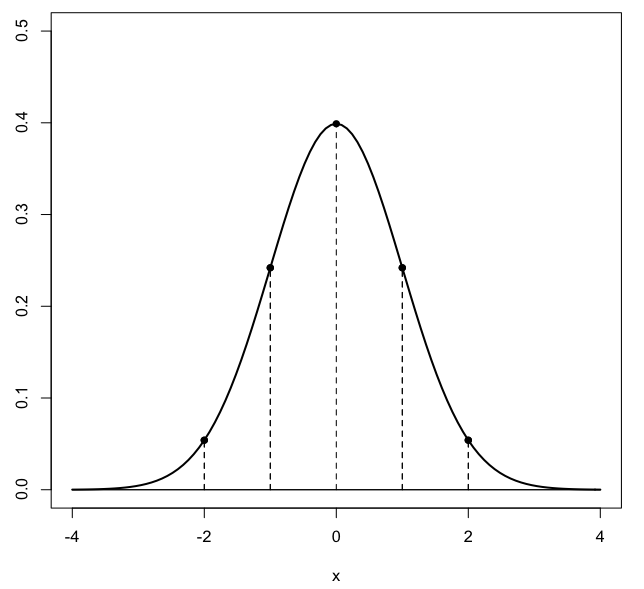
\includegraphics [scale=0.4] {gauss3.png} \end{center}
\begin{document}
\maketitle
\Large
This one is from Ritvik Karkar on Youtube:  Computing Line Integrals

Suppose $f(z) = |z|^2$ and the curve is from $2 + 0i \rightarrow 3 + 1i$.  We should \emph{always} draw a picture, but I'm going to skip it for this one.  This is a straight line which goes across one unit and up one unit.

My way to do this is to say:
\[ |z|^2 = zz* = (x + iy)(x - iy) = x^2 + y^2 \]
That is
\[ u(x,y) = x^2 + y^2 \]
\[ v(x,y) = 0 \]
\[ I = \int u \ dx - \int v \ dy + i \ [ \ \int v \ dx + \int u \ dy \ ] \]
\[ = \int u \ dx + i \int u \ dy \]

Furthermore, along the curve, $y = x - 2$ so $dx = dy$ and
\[ x^2 + y^2 = x^2 + (x - 2)^2 = 2x^2 - 4x + 4 \]
Since $x = 2 \rightarrow 3$ our integral is
\[ \int_2^3 (2x^2 - 4x + 4) \ dx + i \int_2^3 (2x^2 - 4x + 4) \ dx \]
\[ = (1 + i) \int_2^3 (2x^2 - 4x + 4) \ dx \]
\[ = (1 + i) \ [ \ \frac{2}{3} x^3 - 2x^2 + 4x \ ] \ \bigg |_2^3 \]
The term in brackets is
\[ \frac{2}{3}(3^3 - 2^3) - 2(3^2 - 2^2) + 4 \]
\[ = \frac{38}{3} - 10 + 4 = \frac{20}{3} \]
So the final answer is $(1+i) \cdot 20/3$.
\subsection*{alternatively}
His method is to first start with a parametrization with $t = [0,1]$.  So the curve is "start point plus (end point - start point) times t".  The start point is $2 + 0i$, while the end minus the start is $(1+i)$.  Hence
\[ \gamma(t) = (2+0i) + (1+i)t = (2 + t) + i t \]
So everywhere along the curve $z = \gamma(t)$.  Now evaluate the integral as
\[ \int_{\gamma} f(\gamma(t)) \ \gamma'(t) \ dt \]
The function is 
\[ |z|^2 = |\gamma(t)|^2 \]
\[ = (2+t)^2 + t^2 = 4 + 4t + 2t^2  \]
(just using the complex conjugate). 

The derivative is
\[ \gamma'(t) = (1 + i) \]
Our integral is
\[ \int_0^1 (4 + 4t + 2t^2) (1+i) \ dt \]
Notice that $(1+i)$ is just a number
\[ = (1+i) \int_0^1 4 + 4t + 2t^2 \ dt \]
The integral is
\[ 4t + 2t^2 + \frac{2}{3} t^3 \ \bigg |_0^1 \]
Evaluation is easier because the limits are $0 \rightarrow 1$:
\[ = 6 + \frac{2}{3} = \frac{20}{3} \]
Putting it all together we have
\[ (1+i) \cdot \frac{20}{3} \]

\subsection*{another example}
Another typical parametrization is a circle or part of a circle.  Suppose we are on the unit circle starting at $1$ and curving counter-clockwise through $i$ and ending at $-1$.

Use $t$ as our parameter, so 
\[ \gamma(t) = e^{it} \]
\[ \gamma'(t) = i e^{it} \]
with $t = [0, \pi]$.  Looking at the function $f(z) = z^2$ (subtly different than last time) we have
\[ \int_{\gamma} z^2 \ dz = \int_0^{\pi} e^{i2t} \ i \ e^{it} \ dt \]
\[ = i  \int_0^{\pi} e^{i3t} \ dt \]
\[ = i \ \frac{1}{3i} \ e^{i3t} \ \bigg |_0^{\pi} = \frac{1}{3} \  [ \ e^{i3 \pi} - 1 \ ] \ \]
where
\[ e^{i3 \pi} = \cos 3 \pi + i \sin 3 \pi = -1 \]
Hence the final answer is $-2/3$.

\end{document}  